\documentclass[twoside,a4paper,12pt,english]{inac19}

%INAC2017 SETUP: SET PAGE SIZE AND SET FOR USING graphicx PACKAGE.
\usepackage{graphicx}
\usepackage{babel,varioref,epsfig} %,rotating}
\usepackage{amssymb}
\usepackage[font=bf,center]{caption}
\usepackage{subfigure}

\usepackage{textcomp}             % Para usar marca registrada

%\title{MANAGING AND USING A PROFESSIONAL CLUSTER IN NUCLEAR ENGINEERING APPLICATIONS}
\title{THE LTHN COMPUTER CLUSTER}

%INAC2017 SETUP: SPECIFY AUTHOR NAMES, AFFILIATION, ADDRESS AND E-MAIL.

\author{
  \bf{Vitor Vasconcelos, Andr\'e dos Santos,}\\
  \bf{Daniel Campolina and Graiciany Barros}\\ \\
  CDTN - Centro de Desenvolvimento da Tecnologia Nuclear\\
  Av. Ant\^onio Carlos 6627 - Campus UFMG\\
  31270-901 - Belo Horizonte, MG\\
  \{vitors, aacs, campolina, graiciany.barros\}@cdtn.br}


}
\begin{document}

%INAC2017 SETUP: PRINT TITLE
\maketitle

% Acrescentado para facilitar a redação da NI associada
%\tableofcontents
%\tableofcontents


%INAC2017 SETUP: SETUP HEADS FOR PAGES
\pagestyle{myheadings}
\thispagestyle{empty}
\markboth{}{}


%INAC2017 SETUP: SET FIRST PAGE WITH NO PAGE NUMBER
\thispagestyle{empty}

%--------------------------------------------------------------------------------------
\begin{abstract_full_paper}
Computers have become a fundamental tool at almost every human activity.
In science, they're ubiquitous and used so widely that are often neglected
as a complex tool. A professional computer cluster is a good example of
this situation. Many high-end computers in expensive hardware configuration
put together using state-of-the-art software tools usually overlooked by
users as a 'set of computers'. In this paper we present such scientific tool
in a particular context: a high-end cluster system installed, managed and operated
by the very same scientific team which employs it on research on the field of Nuclear Engineering.
This work describes the main features of the LTHN/CDTN (Thermal-hydraulics and Neutronics
Laboratory/Nuclear Technology Development Center), considering software solutions
adopted, the impact of it on research currently carried on at the same laboratory
and the future possible applications of the system. A special attention is given to
the distributed file-system, a fundamental feature to allow high-performance in a system
with many physical disk storage units and to the monitoring system. The latter being
the 'eyes' of the users into the system's load and performance. All solutions adopted for the
cluster are based on open or free software and almost the totality of the research
software used is also open or free. Definitely the path towards less expensive
research, a theme of special interest for scientists and researches from developing countries.
\end{abstract_full_paper}

%--------------------------------------------------------------------------------------
\section{INTRODUCTION}\label{int}

{\Huge Cheio de partes do outro paper!}\\
{\Huge Conferir com cuidado!}\\



%--------------------------------------------------------------------------------------
\subsection{Context}


%------------------------------------------------------------------------------
\section{OBJECTIVE}

The objective of this work is to present the current status of the cluster equipament 
at the Laboratory of Thermal-hydraulics and Neutronics of CDTN (\textbf{LTHN}), describing the decisions 
taken during the installation process, the solutions applied to common (and uncommon) problems 
derived from running a professional cluster system. Together with technical decisions, the 
performance of the system is asserted by comparison to the older system used by the laboratory 
team. 

%------------------------------------------------------------------------------
\section{METHODS AND PROCEDURES}

Main information to be detailed: the cluster uses hostbased authentication, GPU used via 
vnc, \texttt{data} directory at each user account pointing to gluster, how many gluster 
volumes (why two, how they are configured - distributed) and what each one stores, 
the NAS configuration (related to the cluster).

Must update the old figures accordingly. Pehaps add two more figures showing NAS 
and on the internal structure of gluster/NAS.

List the applications running (if possible with some benchmarks) and installed. 
Future work, if something is still missing.

%------------------------------------------------------------------------------
\subsection{Local Structure}
CLUSTER, NAS, NOBREAK, OTHER HARDWARE

Falar da instalação do pacote lm\_sensors para permitir o controle de temperatura dos núcleos. Vale fazer um gráfico para mostrar o quanto sobe 
a temperatura durante uma simulação Monte Carlo com o MCNP.

%In order to start the operation of a cluster system, there are some considerations the must
%be taken in account. The physical location of the system is fundamental for safe, secure and
%reliable operation.

%From the security point of view, the cluster is located at a locked room with limited access to
%the personal related to manage and install the system. The building in which the cluster is located
%is part of the entire institute which is fenced and guarded by armed security personal, what makes
%unauthorized access or intrusion a minor issue.

%The meaning of safety in this text is related to only to system safety. Personal
%safety is not an issue since no special conditions are necessary to operated and use the cluster other
%than use an ordinary desktop computer. The safety of the system consist in guarantee environmental conditions
%which are not harmful to the hardware. In order to guarantee a proper operational temperature, two dedicated
%air conditioning devices work in parallel. These equipments are dimensioned to be able to maintain, each one alone,
%the working temperature at the cluster room considering the system at full operation, i.e. all nodes using all cores
%and GPUs.

%Related to reliability, the system is plugged to a remotely configurable no-break of 40KvA. This equipment
%can provide power for the whole cluster for more than 10 minutes, time enough to be able to save the state of current jobs
%for all users. The implementation of shutdown scripts related to no-break signals is still to be defined.

%------------------------------------------------------------------------------
\subsection{Hardware}


\begin{figure}[h] % t forces top and b forces bottom: can be added to h, ex. [ht]
  \centering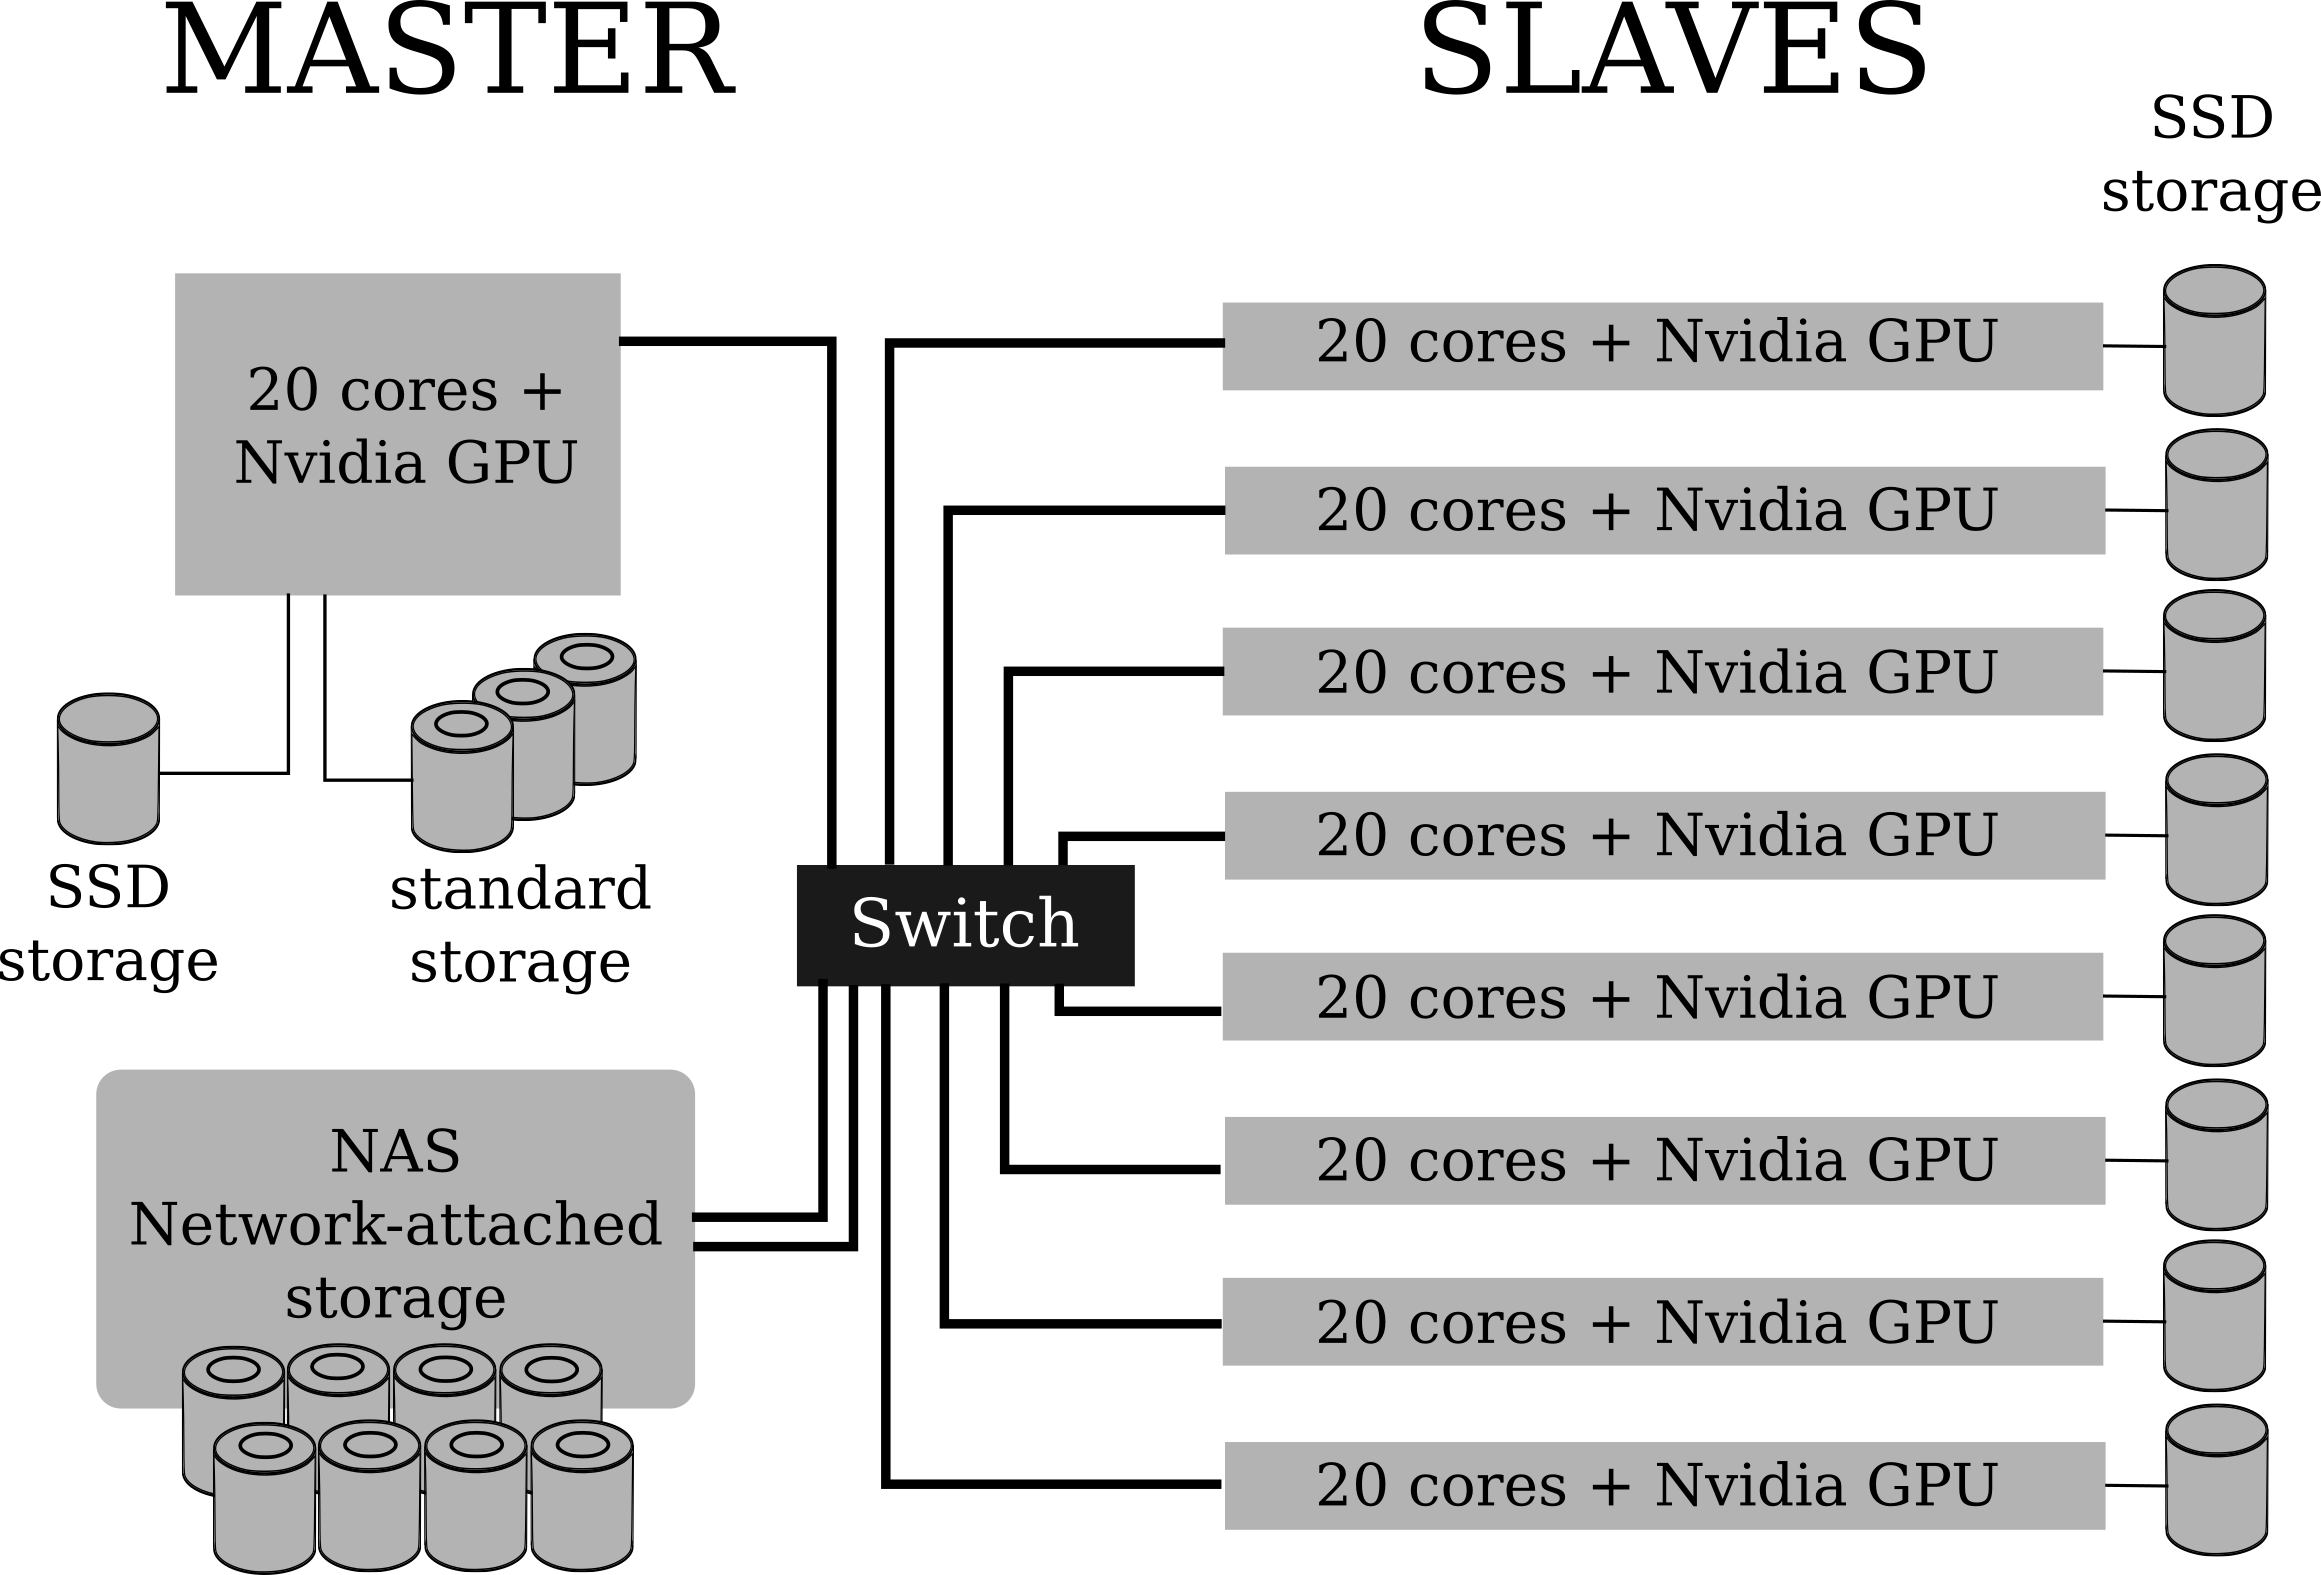
\includegraphics[scale=0.7]{images/cluster-topologico.png}
  \caption{Cluster hardware.}
  \label{fig:cluster}
\end{figure}

The \textit{slaves} are Dell workstations Precision R7910 equipped
with Dual Intel{\textregistered} Xeon{\textregistered} processors E5-2640 operating at $2.4$GHz with
$32$Gb of RAM each. They have two $10$GbE (Gigabit Ethernet) and also two $1$Gbit network connectors, which
allow the use of the Gigabit network exclusively for intra-cluster communication. Their disks are $360$Gb SSD
and are used to store the Operating System of each node and also part of the \textit{Gluster} distributed
file system. These equipments are also installed with Nvidia{\textregistered} GPUs (Graphic Processing Units) M4000{\textregistered} with $8$Gb CUDA\cite{CUDA} capable.

The GPUs on nodes are used as calculation units by the software which can take advantage of this kind of hardware.
It is worth mentioning the increase on the use of GPUs - commonly called accelerators - in scientific computing
in the recent years\cite{accelerators}.

The \textit{master} node is a Dell Precision T7910. The main
differences between the \textit{master} node and the \textit{slaves} machines are two: the \textit{master} has
a slightly worst graphics card, a Quadro{\textregistered} M2000 with $4$Gb of memory. However, the second difference
is the ammount of RAM memory. The nodes are equipped with $32$Gb of memory whereas the \textit{master} has
$256$Gb of RAM.

The master node also have three hard-disks of $500$Gb used as part of the distributed file system, offering
an extra $1.5$Tb of storage for the system as a whole.



%--------------------------------------------------------%
%The original OS sold with the cluster is an OEM (Original Equipment Manufacturer) Windows 7{\textregistered}\cite{windows7}. This
%OS is not supported by the whole set of software expected to be used by the research group users. The chosen
%system to replace the original Windows 7 is CentOS (Community Enterprise Operating System)\cite{centos}, which offers a platform to natively run all
%software needed by the users. CentOS is a community driven free-software effort which focuses in provide a robust open source ecosystem.
%Its typical users are organizations or individuals which have professional oriented hardware but do not need strong commercial support
%in order to achieve successful operation. It is fully compatible with Red Hat Enterprise Linux and in full compliance with Red Hat's
%redistribution requirements.

%Details on possible options for software compatibility and operating system independence will be given on subsections \ref{ssub:dock} and \ref{ssub:virt}

%------------------------------------------------------------------------------
\subsection{Linux Operating System}

%The reason for choosing \textit{CentOS} as the Linux flavor for the system is due to its characteristics and the previous
%experience of the cluster management team. CentOS is aimed to offer a free, enterprise-class, community-supported computing
%functionality. It appeared as a fork of Red Hat Enterprise Linux, which is available only trough paid subscription. The option
%for CentOS, in this context, is to have both the strong development for enterprise systems and also its gratuity.

%A second reason is to take advantage of previous competence of the installation and user team which already has experience
%in using Fedora Linux, a distribution fully compatible with CentOS.

%That said, all the software currently in use by the Thermal-Hydraulics Laboratory team are compatible with CentOS. This
%makes this flavor of Linux the straightforward choice for the cluster system. It is also worth noting that the use of
%free and open-source software has a social meaning in promoting the share of knowledge.

%------------------------------------------------------------------------------
\subsection{Software Solutions}
\label{sub:ssol}


%Before choosing a software for perform a desirable task, its mandatory to have a consistent definition of the environment
%in which the system will be used. The first constraint is the network environment. It's worth noting that the cluster is
%located in the CDTN network and the restrictions and security rules enforced in the network must be followed by the system.

%With this is mind, the choice is to have the main system - interchangeably called slave machines or cluster nodes - in one isolated sub-network only accessed by
%the master node. The master node is part of both the sub-network and the institute's network. The sole point of access to the
%internet for any slave is the master node which, in turn, is connected to the internet using a proxy connection and a
%NAT (Network Access Translation). The topology of the cluster network is presented in Figure~\ref{fig:esquema-cluster}.

\begin{figure}[h] % t forces top and b forces bottom: can be added to h, ex. [ht]
%  \centering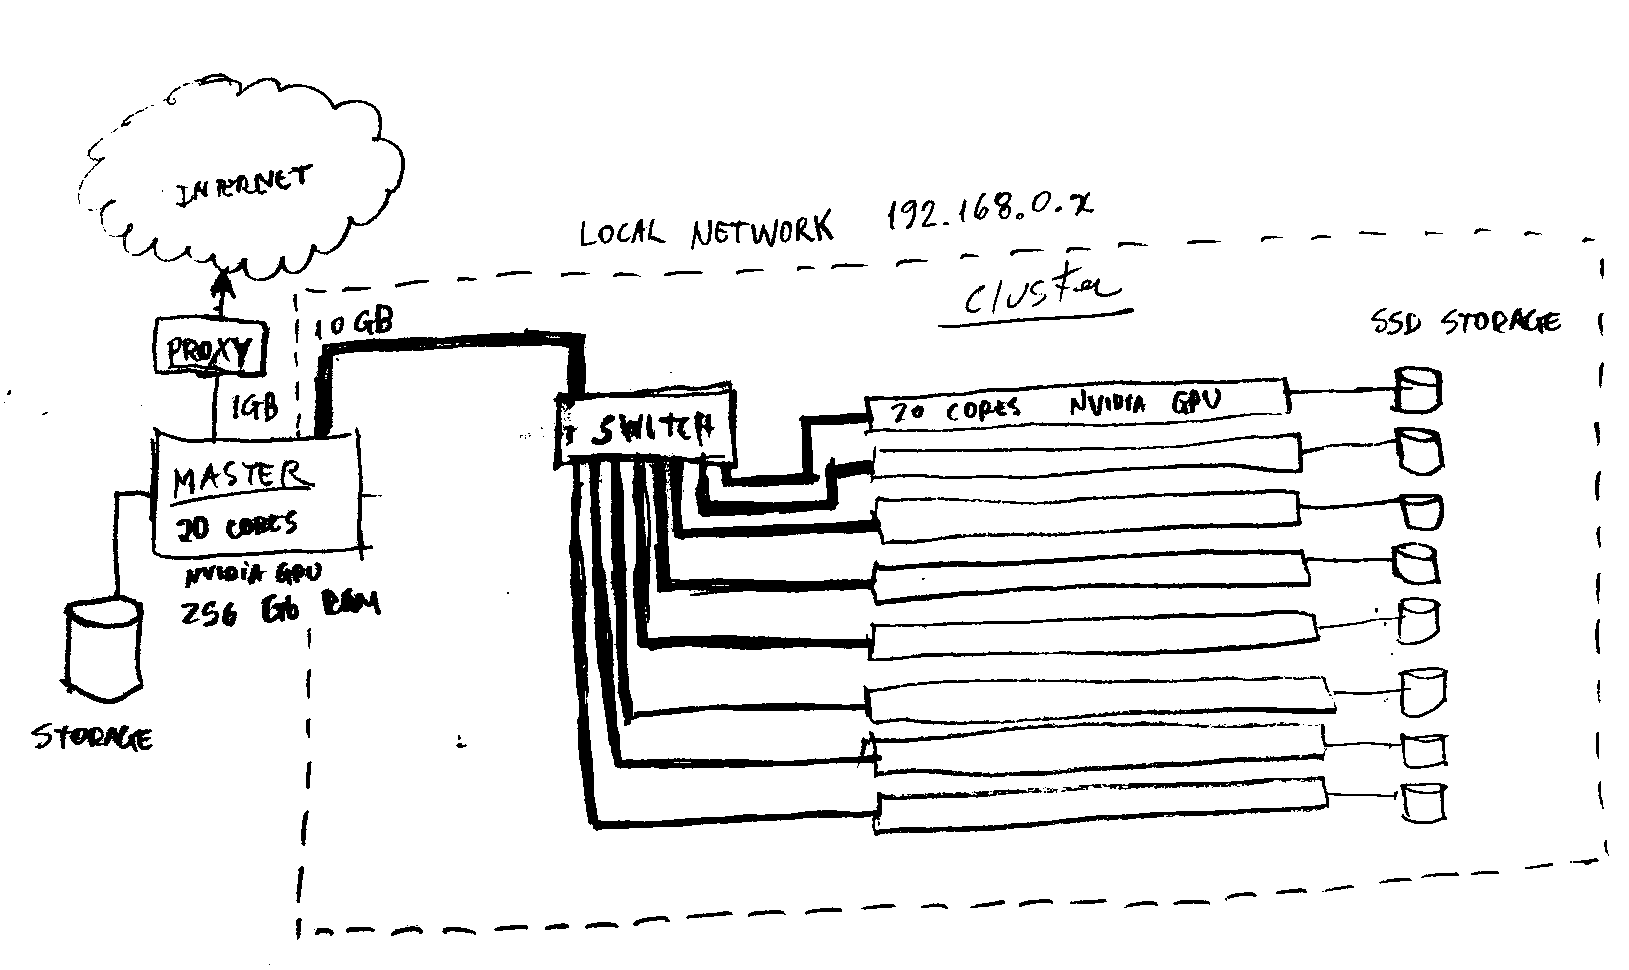
\includegraphics[width=8.5cm,height=8.5cm]{images/esquema_cluster_edited_bw.png}
  \centering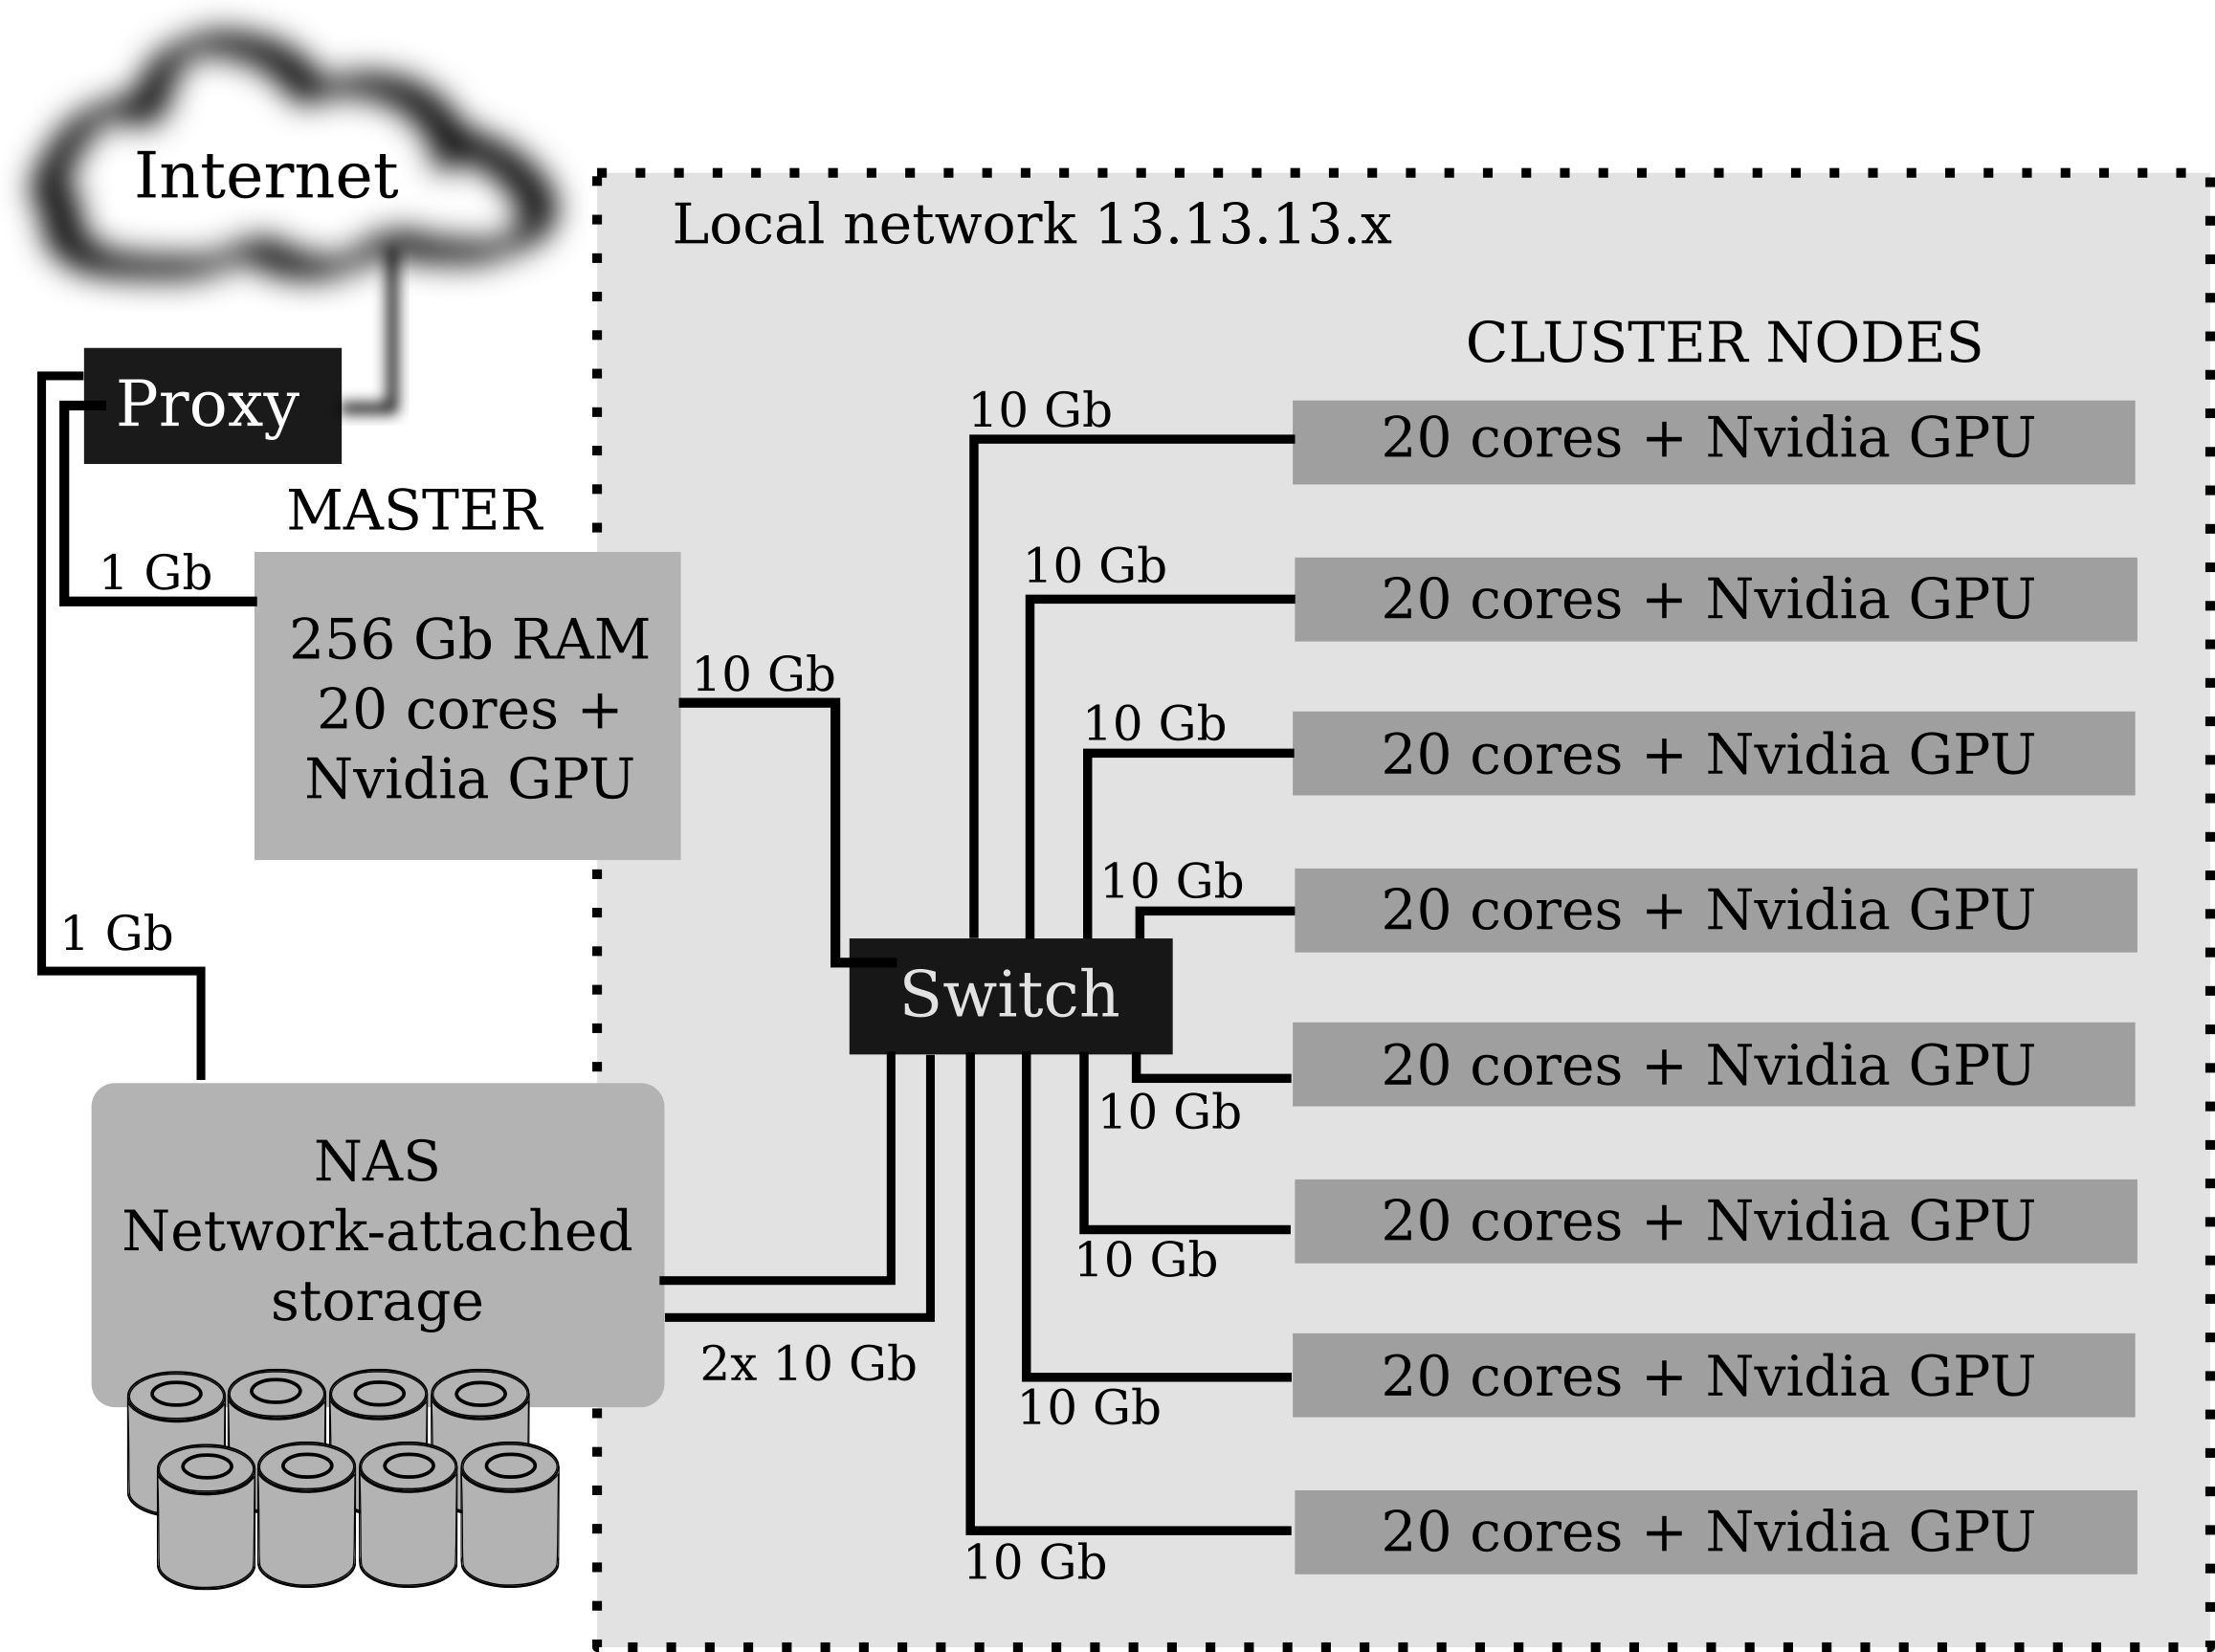
\includegraphics[scale=0.7]{images/cluster-rede.png}
  \caption{Cluster showing its network topology.}
  \label{fig:esquema-cluster}
\end{figure}

%The chosen network topology have impacts on system maintenance. Since the slave machines cannot access the internet, the
%master is configured to hold a mirror of packages installed in all system machines. The average download rate for main CentOS package provider site at the
%master node is of $500$Kbytes/second in trough the proxy in CDTN's network.
%With this in mind, the master machine is scheduled to make updates from time to time (once a week in the current configuration) while the slaves are also scheduled to
%make their updates after the master and from master's local repository. This approach has advantages, like decreasing internet bandwidth demand since only
%one machine downloads updated packages from the internet. Other advantage is in downloading time, since the slaves
%use dedicated $10$GbE connections to the master which provides the necessary packages.

%As expected, this approach has its drawback. A certain amount of disk space is needed to keep a mirror of CentOS packages locally.
%To decrease this space consumption, only packages already installed on the system - master and slaves - are
%downloaded and kept in the local repository. In the case of the installation of a new package not yet present in the repository,
%it must be installed in the master. After that, the scheduled script guarantees its availability for the slaves. In the uncommon
%situation where a package is necessary for the nodes but not for the master, it must be manually added to the repository. This task
%is facilitated by CentOS packages manager \verb yum \cite{yum}

%However, there are more than one way of setup a cluster system with respect
%to file system, software execution and user access.

%The next sub-sections describe alternatives to the use of a direct installation of CentOS version of Linux operating system.
%They are not currently in use in the describe cluster system, but are presented in this paper as they remain as alternatives
%or complementary options for specific cases. For example, the use of a software which is incompatible with another one already
%in use.


%------------------------------------------------------------------------------
\subsection{File System}

During the installation phase of the cluster system\cite{cluster17} were two the contenders for
distributed filesystem solution. The chosen one is described below.

%------------------------------------------------------------------------------
\subsubsection{Gluster File System}

GlusterFS\cite{gluster} is an open source, distributed file system and has
a unique no-metadata server architecture. This is the chosen solution for the system due to its relatively
small number os physical disks and nodes (nine).

The system is configured to use two gluster volumes, namely \texttt{gv-apps} and \texttt{gv-data}. Both volumes
are configured as \textit{distributed} without replication. Since the whole system has an extra NAS device, there is
no need of keeping redundant data. The \texttt{gv-data} offers $N$ Gb of storage per user and is used to run simulations or any task that needs storage during execution. After that, data must be moved to a storage space on NAS where an automatized regular backup avoids data loss.


%------------------------------------------------------------------------------

\section{RESULTS AND ANALYSIS}

%------------------------------------------------------------------------------

\section{CONCLUSIONS AND PERSPECTIVES}

%(O que está bom, o que está ruim na atual instalação)
%(Trabalhos futuros: pra onde ir (operação), possíveis mudanças)

%The process of acquiring, installing and managing a cluster system is a very specific task aimed to well trained
%personal. In a perfect situation, a team of specialists would take care of these tasks letting the users - scientists in the present case -
%free to focus on their research work and on how to take the most of such system. However, in other cases the users themselves must
%take care of the whole process.

%Although challenging, this can be seen as an opportunity to have a deeper of understanding of the tool one must use the accomplish his tasks.
%This the case in this work, where the users had to chose among many options to make a professional cluster operational.

%As an ongoing work, some of the challenges - like defining and installing a distributed file system, for example - were successfully
%addressed. Other remain to be figured out and worked out.

%There are many ongoing tasks and even more tasks still to be started. To mention a few, one
%interesting task related to the reliability and data management is the implementation of
%a automatic process of shutdown on loss of power supply. Other one is to define a systematic
%user account backup to avoid loss of data of expensive simulations at the same time ensuring
%disk space availability.

%As a conclusion, there is a clear trade-off between the situation where the tool - at the limit, a complex tool like a cluster is a tool - is available and ready to use and
%the discussed case in this paper. The former clearly saves precious time that scientists can devote to their research work itself. However, the latter situation has a not so obvious
%advantage: being forced to expend time to understand details of the cluster operation, scientists can acquire a new perspective on how to apply their
%methods. This can lead to changes or improvements in the way a problem is solved. If this is a real advantage is yet to be shown. However,
%in a situation like the one presented, where there is no choice, this can be seen as a positive condition on the improvement of methods, solutions and approaches used
%uncritically on a daily basis.


%Uma cita\c{c}\~{a}o \cite{Henderson17}.


%------------------------------------------------------------------------------



\section*{Acknowledgments}
The authors would like to thank FUJB for financing the cluster acquisition
as part of the project \textit{Desenvolvimento de novos elementos combust\'{i}veis nucleares
  e materiais e pe\c{c}as para combust\'{i}veis nucleares}, agreement FINEP 01.07.0548.00 - Process FUJB 13.867-3.
The authors also thank Dr. Jo\~{a}o Roberto Loureiro de Mattos, now retired, for the work which made possible the acquisition of the cluster.

%%%%%%%%%%%%%%%%%%%%%%%%%%%%%%%%%%%%%%%%%%%%%%%%%%%%%%%%%%%%%%%%%%%%%%%%%%%%%%%%%%%%%%%%%%%%

\begin{thebibliography}{99} %99 é o número máximo que o thebibliography permite. Numero de referencias que aparecerão.

\bibitem{linux} ``The Linux Documentation Project'', \\\verb#http://www.tldp.org/LDP/intro-linux/html/chap_01.html# (2017).

\bibitem{Dongarra2017} John Dongarra et. al., ``With Extreme Computing, the Rules Have Changed'', \textit{Computing in Science Engineering}, \textbf{19}, pp. 52--62, (2017).

\bibitem{CUDA} John Nickolls, Ian Buck, Michael Garland and Kevin Skadron, ``Scalable Parallel Programming with CUDA'', \textit{Queue - GPU Computing}, \textbf{6}, pp. 40--53, (2008).

\bibitem{accelerators} ``What is GPU-accelerated computing?'', \\\verb#http://www.nvidia.com/object/what-is-gpu-computing.html# (2017).

%\bibitem{windows7} Jorge Orchilles, \textit{Microsoft Windows 7 Administrator's Reference}, Syngress, Boston USA (2010).
  
  % Centos
\bibitem{centos} ``The CentOS Project'', \verb#https://www.centos.org# (2017).

\bibitem{yum} ``man7.org yum man page'', \verb#http://man7.org/linux/man-pages/man8/yum.8.html# (2017).
  
\bibitem{Boettiger} Carl Boettiger, ``An introduction to Docker for reproducible research'', \textit{SIGOPS Operating System Review}, \textbf{49}, pp. 71--79, (2015).

\bibitem{Tommaso} Paolo Di Tommaso et al. ``The Impact of Docker Containers on the Performance of Genomic Pipelines'' \textit{PeerJ}, \textbf{3}, (2015).

  % Virtualizacao (9 e 10)
\bibitem{vir1} A. J. Younge and G. C. Fox, ``Advanced Virtualization Techniques for High Performance Cloud Cyberinfrastructure'', \textit{2014 14th IEEE/ACM International Symposium on Cluster, Cloud and Grid Computing}, Chicago, IL, USA, pp. 583--586, May, (2014).
  
\bibitem{vir2} I. Sadooghi, J. H. Martin, T. Li, K. Brandstatter, K. Maheshwari, T. P. P. de Lacerda Ruivo, G. Garzoglio, S. Timm, Y. Zhao and I. Raicu, ``Understanding the Performance and Potential of Cloud Computing for Scientific Applications'', \textit{IEEE Transactions on Cloud Computing}, \textbf{5}, pp. 358--371, (2017).
  
\bibitem{linuxbook} Wirzenius and Lars, \textit{The  Linux System Administrator's Guide}, iUniverse incorporated (2000).

\bibitem{hal} Benjamin Depardon, Ga\"{e}l Le Mahec and Cyril S\'{e}guin, ``Analysis of Six Distributed File Systems'', Research Report, pp. 44, (2013).
  
\bibitem{gluster} Alex Davies and Alessandro Orsaria, ``Scale out with GlusterFS'', \textit{The Linux Journal}, \textbf{2013}, (2013).

%\bibitem{lustre} ``Lustre* Software Release 2.x: Operations Manual'', Editor: Intel Corporation, (2017).

\bibitem{paraview} Ayachit, Utkarsh, \textit{The ParaView Guide: A Parallel Visualization Application}, Kitware, ISBN 978-1930934306, (2015).

\bibitem{gpgpu}  John D. Owens, David Luebke, Naga Govindaraju, Mark Harris, Jens Kr\"{u}ger, Aaron E. Lefohn, and Tim Purcell, ``A Survey of General-Purpose Computation on Graphics Hardware'', \textit{Computer Graphics Forum}, \textbf{26(1)}, pp. 80--113, March (2007).

\bibitem{opencl} J. E. Stone, D. Gohara and G. Shi, ``OpenCL: A Parallel Programming Standard for Heterogeneous Computing Systems'', \textit{Computing in Science \& Engineering}, \textbf{12(3)}, pp. 66--73, May-June (2010).

\bibitem{cluster17} Vitor V. A. Silva, André A. C. dos Santos and Renan O. Cunha, ``Professional Cluster Management
    by a small scientific team: challenges, solutions and perspectives'', \textit{XX ENFIR INAC 2017 International Nuclear Atlantic Conference }, Belo Horizonte, MG, Brazil, pp. xx-yy, October, (2017). 

\end{thebibliography}

% ---------------------------------------------------------
% Minha bibliografia usando arquivo externo
%\bibliographystyle{unsrt}
%\bibliography{bibli}


\end{document}
